\documentclass{article}


\usepackage{arxiv}

\usepackage[utf8]{inputenc} % allow utf-8 input
\usepackage[T1]{fontenc}    % use 8-bit T1 fonts
\usepackage{hyperref}       % hyperlinks
\usepackage{url}            % simple URL typesetting
\usepackage{booktabs}       % professional-quality tables
\usepackage{amsfonts}       % blackboard math symbols
\usepackage{nicefrac}       % compact symbols for 1/2, etc.
\usepackage{microtype}      % microtypography
\usepackage{lipsum}
\usepackage{amsmath}
\usepackage{graphicx}

\title{Taming VAEs\\
\normalsize{Bayesian Methods of Machine Learning 2018}}


\author{
  Anna Kuzina   
    \And
  Denis Prokopenko
    \And
  Valentina Shumovskaia
}

\begin{document}
\maketitle

\section{Problem}

Deep variational auto-encoders (VAEs) have made substantial progress in the last few years on modelling complex data such as images, speech synthesis, molecular discovery, robotics and 3d-scene understanding. The most popular method for training these models is through stochastic amortized variational approximations, which use a variational posterior to construct the evidence lower-bound (ELBO) objective function.

Our main goal is to implement an approach proposed by Danilo J. Rezende and  Fabio Viola \cite{taming}. The main question is: whether this approach is really better than \cite{vae} or \cite{betavae}? We did experiments with VAE, $\beta$-VAE, GECO algorithm, compared them on MNIST and CIFAR-10 data sets. The next goal is to try to improve this approach by combining this method and \cite{iwae1}, \cite{iwae2}. Such a model was implemented and compared with the others on MNIST data set.

\subsection{VAE and $\beta$-VAE}

We solve the following optimization problem:
\begin{equation}\label{eq:VAE}
    \mathkal L(\theta, \phi, x^{i}) = -\beta D_{KL}(q_{\phi}(z|x^{(i)})||p(z)) + \mathbb E_{q_{\phi}(z|x^{(i)})}(\log p_\theta (x^{(i)}|z)),
\end{equation}
where $x$ is a data, $z$ is a latent space, $p(z)$ is a latent distribution. The specific case $\beta = 1$ is an initial VAE model, $q_{\phi}$ is an encoder, $p_\theta$ is a decoder.

\subsection{GECO}
Danilo J. Rezende at al. in \cite{taming} offered to take a look at this problem from another point of view, which helps to treat $\beta$ as a trainable parameter. The idea is problem of ELBO maximization can be reformulated as a conditional minimization problem: find the minimal possible KL-divergence for a given value of a reconstruction loss, with the following Lagrangian:
\begin{equation}\label{eq:Lagrangian}
    KL(q(z|x)\|p(z)) + \lambda^T \mathbb{E}_{q(z|x)}(Re(x, g(z)) \rightarrow min
\end{equation}
Where reconstruction loss can be computed as:
\begin{equation*}
    \|x - g(x)\|^2 - \kappa^2
\end{equation*}

\begin{figure}[!h]
\centering
  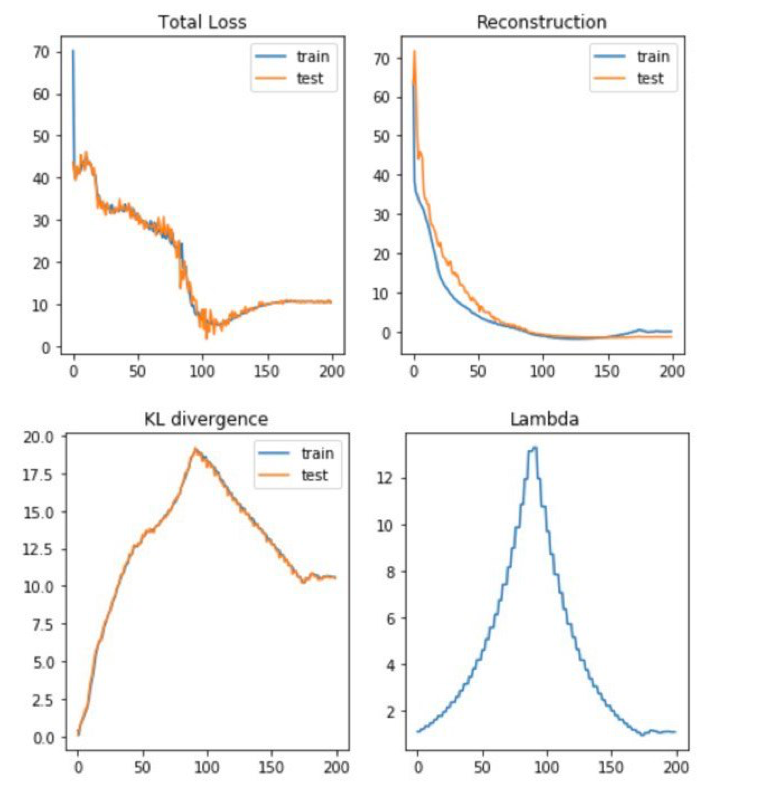
\includegraphics[width=0.5\linewidth]{pics/geco1}
\caption{\label{fig:geco}Training of GECO Algorithm on MNIST}
\end{figure}
  As a result, $\lambda$ is adjusted interactively. At the beginning, when reconstruction is poor, $\lambda$ increases from iteration to iteration. But as soon as reconstruction becomes equal to predefined tolerance level, $\lambda$ stats to fall, resulting it increased weight of KL-divergence in the loss. The run of the algorithm is illustrated on \ref{fig:geco}.

\subsection{IWAE}
Yuri Burda et al. \cite{iwae1} introduced the improvement of variational autoencodes. Instead of (\ref{eq:VAE}) we consider the following variational $k$-sample importance weighting estimate of the log-likelihood with reparametrization trick:
\begin{equation}
    \mathcal{L}_k(x) = \mathbb{E}_{\mathbf{h}_1, \dots, \mathbf{h}_k \sim q(\mathbf{h}|\mathbf{x})}\Big[\log \frac{1}{k} \sum_{i=1}^k \frac{p(x,h_i)}{q(h_i|x)}\Big]
\end{equation}
When $k=1$, $k$-sample importance weighting estimate of the log-likelihood becomes usual VAE estimate log-likelihood. According to the Theorem 1 from \cite{iwae1}:
\begin{equation}
    \log p(x) \geq \mathcal{L}_{k+1} \geq \mathcal{L}_k.
\end{equation}
As a result such estimation increases flexibility to model complex posteriors, which do not fit the VAE modeling assumptions. It may be shown that IWAEs learn richer latent space representations than VAEs, leading to improved test log-likelihood on density estimation benchmarks.

Training procedure is similar to the original, however there appears importance weighting due to differentiation:
\begin{align*}
    &\nabla_\theta \mathcal{L}_k(\mathbf{x}) = \nabla_\theta\mathbb{E}_{\mathbf{h}_1, \dots, \mathbf{h}_k \sim q(\mathbf{h}|\mathbf{x})} \log \frac{1}{k} \sum_{i=1}^k w_i = \nabla_\theta\mathbb{E}_{\mathbf{\epsilon}_1, \dots, \mathbf{\epsilon}_k} \log \frac{1}{k} \sum_{i=1}^k w_i(\mathbf{x}, \mathbf{h}(\mathbf{x}, \mathbf{\epsilon}_i, \mathbf{\theta})) =\\&= \mathbb{E}_{\mathbf{\epsilon}_1, \dots, \mathbf{\epsilon}_k} \nabla_\theta \log \frac{1}{k} \sum_{i=1}^k  w(\mathbf{x}, \mathbf{h}(\mathbf{x}, \mathbf{\epsilon}_i, \mathbf{\theta})) = \mathbb{E}_{\mathbf{\epsilon}_1, \dots, \mathbf{\epsilon}_k} \sum_{i=1}^k \tilde{w}_i \nabla_\theta \log   w(\mathbf{x}, \mathbf{h}(\mathbf{x}, \mathbf{\epsilon}_i, \mathbf{\theta}))\\
    &\tilde{w}_i = \frac{w_i}{\sum_{j=1}^k w_j}
\end{align*}

\section{Discussion}
\subsection{GECO}
The idea of the discussed algorithm is quite logical. But when it came to realization, a few problems appeared. At the beginning of the training  reconstruction loss it too high, resulting in fast increase of $\lambda$. When finally reconstruction converge to some reasonable value, value of $\lambda$ is already too big and KL diverges converges to a higher values that expected. This peculiarity was not discussed in the paper, but we noticed, that the graphs which they present, actually begin from ~800-1000th iteration. So, we assumed, that it would be better to fix $\lambda$ at some low level for the beginning of the training in order to get proper reconstruction.


\subsection{IWAE}
Now, move on to IWAE implementation. The GECO algorithm is assumed to be used. However, the initial IWAE approach cannot be applied straightforward in that case. Hence, the IWAE estimation should be splitted into two parts: reconstruction and KL divergence. Chris Cremer et al. introduced the way to split using $q_{IW}$.
\begin{align*}
    q_{IW} (z|x) = \frac{p,z}{\frac{1}{k}\sum_{j=1}^k \frac{p(x,z_j}{q(z_j|x)}}\\
\end{align*}
Then the considered Lagrangian will have the following form:
\begin{align}\label{eq:Loss_iwae}
    \mathcal{L}oss_{IW} = \lambda \mathbb{E}_z \log p(x|z) + KL(q_{IW}(z|x)||p(z)) = (\lambda-1) \mathbb{E}_z \log p(x|z) + \mathcal{L}_{k}
\end{align}

As a result the network may be trained by decreasing (\ref{eq:Loss_iwae}), which consists of reconstruction error and IWAE log-likelihood. 





\section{Experiments}
\subsection{MNIST}
All in all, the VAE, $\beta-$VAE, VAE and IWAE trained by GECO were tested on MNIST dataset. The model of variational autoencoder consisted of fully connected encoder: $784\rightarrow 512 \rightarrow 256 \rightarrow 200$ and decoder: $200\rightarrow 256 \rightarrow 512 \rightarrow 784$.  Tolerance was equal 4, batch size was equal 2000. Initial $\lambda_{VAE} = 1$ with step  $100$,for  $\beta$-VAE  we fixed $\beta = 0.5$ $\lambda_{IWAE} = 10000$ with step $=100$. In order to compute proper loss function in case of IWAE, the $k=5$ samples were drawn from latent space for each original picture.\\

The GECO algorithm showed better results for VAE and IWAE both compared to standard VAE and $\beta-$ VAE, see fig. \ref{fig:mnist_rec} and table \ref{tab:mnist}. The generation case showed other useful result. The GECO algorithm applied to VAE outperform the IWAE with GECO and showed the best results, while simple VAEs failed.

\begin{table}[]
    \centering
    \begin{tabular}{|l|l|l|}
    \hline
         Model & Marginal KL & Reconstruction loss\\
    \hline
         VAE & 1.5813 & 55.8484\\
         $\beta$-VAE & 10.5938 & 15.1434\\
         GECO & 10.4975 & 14.6269\\
         GECO + IWAE & 1.3640 & 12.9214\\
    \hline
    \end{tabular}
    \caption{MNIST data set}
    \label{tab:mnist}
\end{table}


\begin{table}[]
    \centering
    \begin{tabular}{|l|l|l|}
    \hline
         Model & Marginal KL & Reconstruction loss\\
    \hline
         VAE & 31.9662 & 77.6570\\
         $\beta$-VAE & 59.4998 & 57.9653\\
         GECO & 383.08495 & 11.4413\\
    \hline
    \end{tabular}
    \caption{CIFAR-10 data set}
    \label{tab:cifar10}
\end{table}

\begin{figure}
\centering
  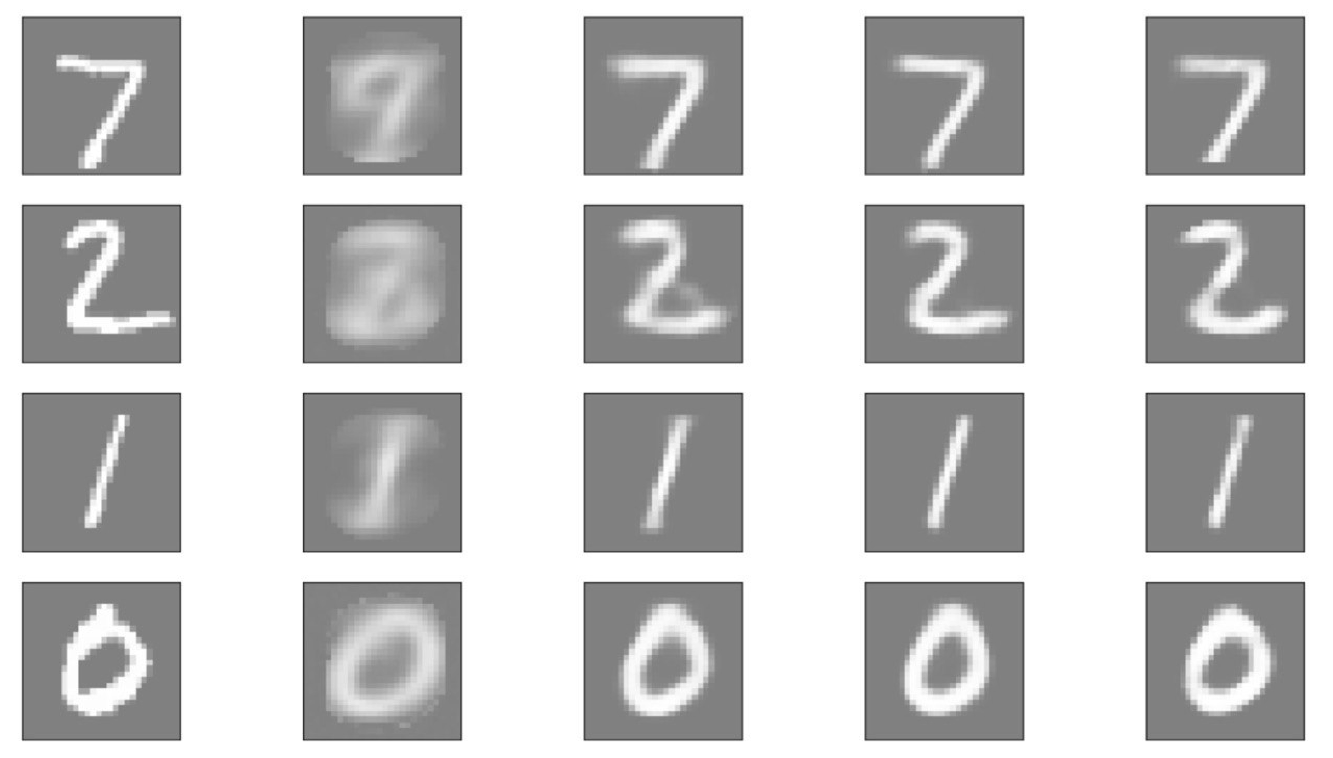
\includegraphics[width=0.5\linewidth]{pics/mnist_rec.png}
\caption{\label{fig:mnist_rec}Ground truth and reconstruction results of VAE, $\beta$-VAE with $\beta=0.5$, GECO, GECO + IWAE models trained on MNIST (from left to right).}
\end{figure}

\begin{figure}[!h]
\centering
  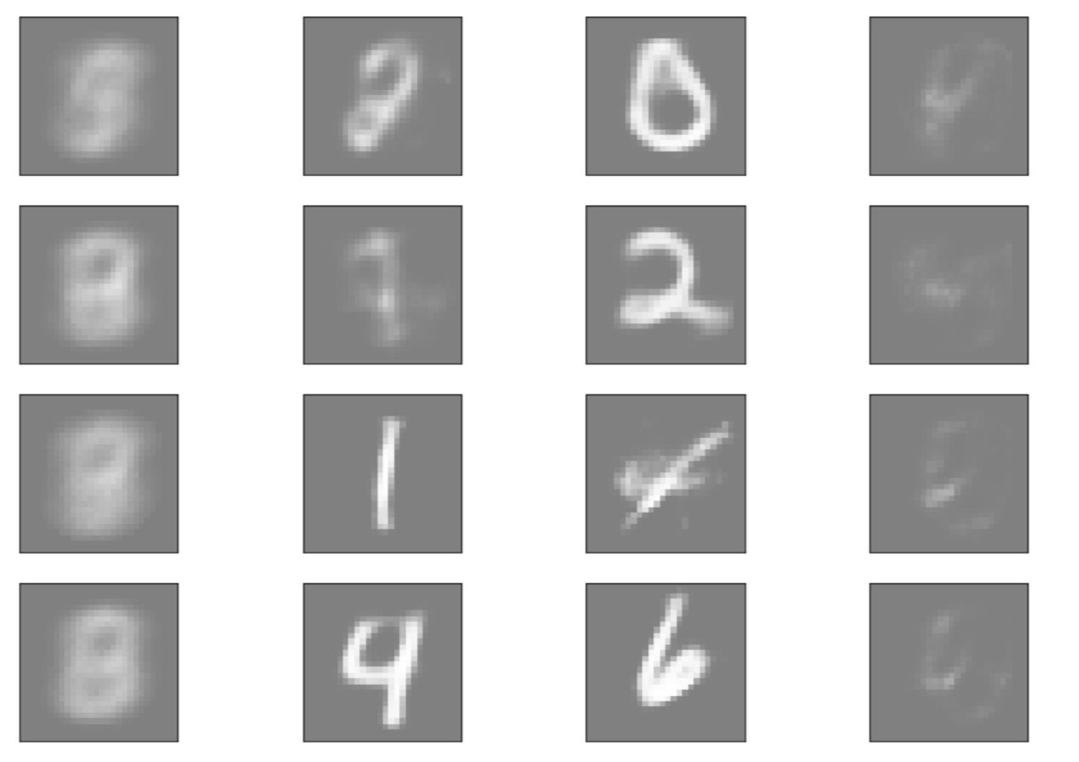
\includegraphics[width=0.5\linewidth]{pics/mnist_gen.png}
\caption{\label{fig:mnist_gen}Generation results of VAE, $\beta$-VAE with $\beta=0.5$, GECO, GECO + IWAE models trained on MNIST (from left to right).}
\end{figure}

\begin{figure}[!h]
\centering
  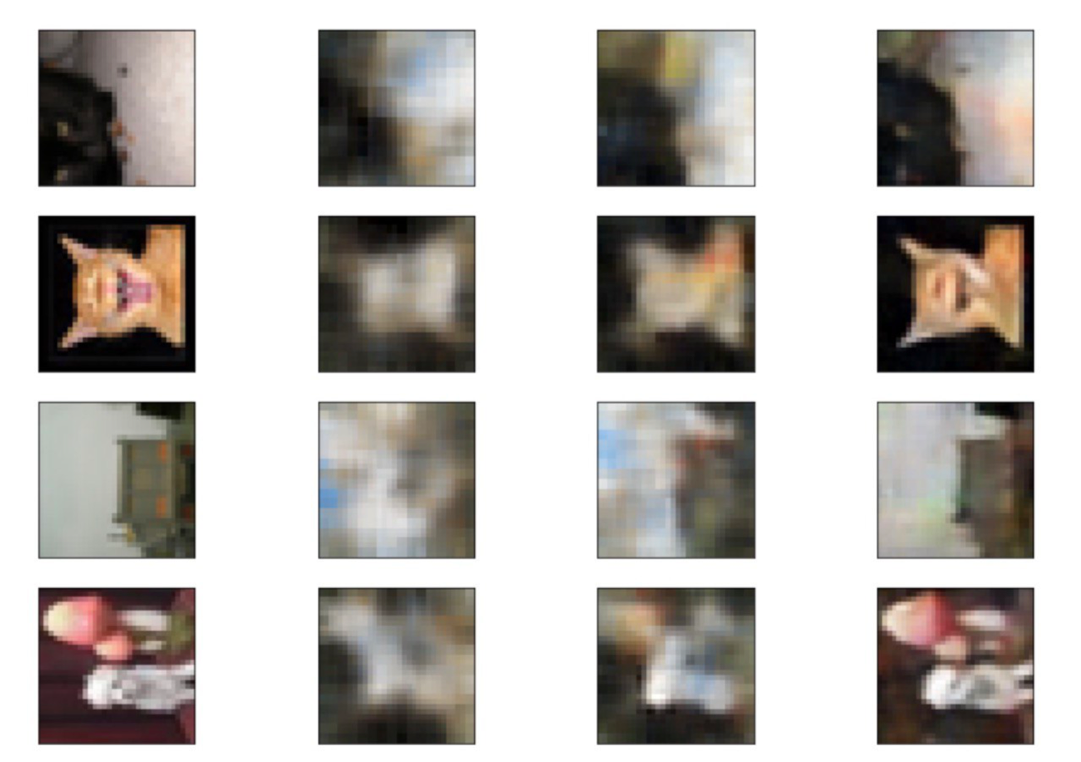
\includegraphics[width=0.5\linewidth]{pics/cifar10_rec.png}
\caption{\label{fig:cifar10_rec}Ground truth and reconstruction results of VAE, $\beta$-VAE with $\beta=0.5$, GECO, GECO + IWAE models trained on CIFAR-10 (from left to right).}
\end{figure}

\subsection{CIFAR10}
For the CIFAR10 dataset, simple fully-connected model did not perform well, therefore, we use ConvolutionalDRAW model instead. It consisted of one LSTM modules, where linear layers were substituted by convolutions. 

To estimate VAE, $\beta$-VAE with $\beta = 0.5$ and GECO-VAE performance, we used hidden dimension of 256 and batch size 300. For GECO we've chosen tolerance of 0.6, which produce nice reconstruction. Initial value of $\lambda = 1$ was adjusted every 100 iterations.

We can see from table \ref{tab:cifar10} and figure \ref{fig:cifar10_rec}, that quality of reconstruction achieved by GECO is much better than the one for simple VAE. But at the same time, posterior density of the latent variables is too far from the prior. It is highly likely, that this is a result of the problem, discussed in the previous part: $\lambda$ grows too fast at the begging, resulting in the extremely complex posterior density, which cannot be simplified further.
\cleardoublepage
\bibliographystyle{unsrt}
\bibliography{references}

\end{document}
